\documentclass[10pt,a4paper,twocolumn]{article}
\usepackage[T1]{fontenc}
\usepackage[utf8]{inputenc}
\usepackage{lmodern}
\usepackage[ngerman]{babel}
\usepackage[margin=2cm,columnsep=0.8cm]{geometry}
\usepackage{microtype}
\usepackage{graphicx}
\usepackage{booktabs}
\usepackage[font=small,labelfont=bf]{caption}
\usepackage[round,authoryear]{natbib}
\usepackage{xcolor}
\usepackage{listings}
\usepackage{tikz}
\usetikzlibrary{positioning,arrows.meta}
\usepackage[hidelinks]{hyperref}
\def\UrlBreaks{\do\/\do-\do.\do_\do=\do?\do\&}
\DeclareUrlCommand\pf{\urlstyle{tt}}
\setlength{\emergencystretch}{3em}
\setlength{\bibsep}{2pt}
\renewcommand{\bibfont}{\small}
\graphicspath{{results/abbildungen/}}
\DeclareUnicodeCharacter{2248}{\ensuremath{\approx}}
\DeclareUnicodeCharacter{2212}{\ensuremath{-}}
\DeclareUnicodeCharacter{2192}{\ensuremath{\rightarrow}}
\DeclareUnicodeCharacter{2265}{\ensuremath{\geq}}
\DeclareUnicodeCharacter{2264}{\ensuremath{\leq}}
\lstdefinestyle{code}{basicstyle=\ttfamily\scriptsize, breaklines=true, columns=fullflexible,
  keepspaces=true, frame=single, rulecolor=\color{black!25}, backgroundcolor=\color{black!3},
  xleftmargin=2pt, xrightmargin=2pt, aboveskip=4pt, belowskip=4pt, showstringspaces=false,
  postbreak=\mbox{{\color{gray}$\hookrightarrow$}\space},
  commentstyle=\color{black!55}\itshape}
\lstset{style=code, extendedchars=true, inputencoding=utf8,
  literate={ä}{{\"a}}1 {ö}{{\"o}}1 {ü}{{\"u}}1 {Ä}{{\"A}}1 {Ö}{{\"O}}1 {Ü}{{\"U}}1
  {ß}{{\ss}}1 {–}{{--}}1 {→}{{$\rightarrow$}}1}

\title{Dokumentation einer Verwandtschafts-Pipeline mit Snakemake:\\
von Ganzgenomdaten zu Mendel-Fehlern und KING}
\author{Karim Andjar\\[2pt]
\small Justus-Liebig-Universität Gießen, Master Bioinformatik und Systembiologie}
\date{\today}

\begin{document}

\makeatletter
\twocolumn[
\begin{@twocolumnfalse}
\maketitle
\renewcommand{\abstractname}{Zusammenfassung}
\begin{abstract}
Diese Dokumentation beschreibt eine vollständige Pipeline, die aus Ganzgenomdaten von vier Personen der CEPH-Familie 1463 ableitet, wer mit wem verwandt ist, ohne dass Rollen vorgegeben werden. Die Verarbeitung läuft als Snakemake-Workflow auf einem Laptop: Herunterladen und Abgleich der Reads, Duplikatmarkierung, Variantenbestimmung im GVCF-Modus, gemeinsame Genotypisierung, Filterung auf verlässliche SNPs und zwei unabhängige Auswertungen, die Zählung von Mendel-Fehlern und der KING-robust-Schätzer. Für jeden Schritt werden die biologische Idee, das Werkzeug, die Snakemake-Regel, die Ein- und Ausgabedateien und die tatsächlich erzielten Zahlen erklärt. Ergänzt wird dies durch die Auswertungsskripte, die vier Abbildungen, eine Anleitung zur Reproduktion und eine Liste der aufgetretenen Probleme mit ihren Lösungen.
\end{abstract}

\renewcommand{\abstractname}{Abstract}
\begin{abstract}
This document describes a complete pipeline that infers relatedness among four members of the CEPH family 1463 from whole-genome data, without assigning roles in advance. A Snakemake workflow runs on a laptop and covers read download and alignment, duplicate marking, GVCF variant calling, joint genotyping, SNP filtering and two independent analyses, Mendelian error counting and the KING-robust estimator. For every step, the biological rationale, the tool, the Snakemake rule, the input and output files and the observed numbers are given, together with the analysis scripts, the four figures, reproduction instructions and a list of problems encountered and their solutions.
\end{abstract}

\noindent\textbf{Schlüsselwörter:} Verwandtschaftsanalyse, Mendel-Fehler, KING, Snakemake, GATK, CEPH 1463
\bigskip
\end{@twocolumnfalse}
]
\makeatother

% ---------------------------------------------------------------------------
\section{Überblick}
Ob zwei Personen verwandt sind, lässt sich aus ihren Genotypen ablesen. Ein Kind erbt von jedem Elternteil genau ein Allel. Elternteil und Kind können deshalb an keiner Position entgegengesetzte Homozygote tragen (AA gegen aa), während das bei nicht verwandten Personen regelmäßig vorkommt. Die Pipeline macht diese Überlegung mit echten Sequenzdaten überprüfbar und leitet die Rollen (Eltern, Kind, nicht verwandt) allein aus den Genotypen ab.

Der Workflow hat drei Teile (Abb.~\ref{fig:schema}). Im ersten Teil werden aus den Reads je Person und Chromosom Varianten bestimmt. Im zweiten Teil werden alle Personen gemeinsam genotypisiert und auf verlässliche SNPs gefiltert, damit alle Vergleiche auf denselben Positionen beruhen. Im dritten Teil werten zwei unabhängige Verfahren die Verwandtschaft aus.

\begin{figure*}[t]
\centering
\begin{tikzpicture}[
  box/.style={draw, rounded corners=2pt, fill=black!4, minimum height=0.9cm, minimum width=2.7cm,
              align=center, font=\small, inner sep=3pt},
  res/.style={box, fill=blue!10, draw=blue!60!black},
  arr/.style={-{Stealth[length=2.2mm]}, thick, black!70},
  node distance=0.55cm]
  \node[box] (a) {FASTQ\\[-1pt]{\scriptsize ENA}};
  \node[box, right=of a] (b) {bwa mem\\[-1pt]{\scriptsize + sort}};
  \node[box, right=of b] (c) {MarkDuplicates};
  \node[box, right=of c] (d) {HaplotypeCaller\\[-1pt]{\scriptsize GVCF je Chrom.}};
  \node[box, right=of d] (e) {CombineGVCFs};
  \node[box, below=1.6cm of a] (f) {GenotypeGVCFs};
  \node[box, right=of f] (g) {bcftools\\[-1pt]{\scriptsize setGT + SNP-Filter}};
  \node[box, right=of g] (h) {concat\\[-1pt]{\scriptsize snps.vcf.gz}};
  \node[res, right=of h, yshift=0.5cm] (i) {Mendel-Fehler\\[-1pt]{\scriptsize mendel.tsv}};
  \node[res, right=of h, yshift=-0.5cm] (j) {KING\\[-1pt]{\scriptsize king.kin0}};
  \draw[arr] (a)--(b); \draw[arr] (b)--(c); \draw[arr] (c)--(d); \draw[arr] (d)--(e);
  \draw[arr] (e.south) -- ++(0,-0.4) -| (f.north);
  \draw[arr] (f)--(g); \draw[arr] (g)--(h);
  \draw[arr] (h.east) -- ++(0.25,0) |- (i.west);
  \draw[arr] (h.east) -- ++(0.25,0) |- (j.west);
\end{tikzpicture}
\caption{Aufbau der Pipeline. Teil 1 (obere Reihe): Reads bis GVCF. Teil 2 (untere Reihe links): gemeinsame Genotypisierung und Filter. Teil 3 (blau): Auswertung. Die Schritte FASTQ bis MarkDuplicates entfallen für Proben, für die eine fertige BAM vorliegt.}
\label{fig:schema}
\end{figure*}

% ---------------------------------------------------------------------------
\section{Umgebung und Installation}
\subsection{Rechner und Software}
Die Pipeline läuft auf einem MacBook Air in einer conda-Umgebung mit dem Namen \texttt{trio\_test}. Alle Programme stammen aus den Kanälen \texttt{bioconda} und \texttt{conda-forge} (Tab.~\ref{tab:sw}). Der Workflow ist mit Snakemake \citep{molder2021} umgesetzt.

\begin{table}[t]
\centering
\small
\caption{Verwendete Software (getestete Versionen).}
\label{tab:sw}
\begin{tabular}{@{}lll@{}}
\toprule
Programm & Version & Aufgabe\\
\midrule
Snakemake & 9.27.0 & Workflow\\
bwa & 0.7.19 & Abgleich\\
samtools & 1.24 & Sortieren, Index\\
GATK & 4.6.2.0 & Duplikate, Varianten\\
bcftools & 1.24 & Filter, Zusammenfügen\\
PLINK 2 & 2.0.0a.7.8 & KING\\
Python & 3.11.17 & Auswertung\\
Matplotlib & 3.11.2 & Abbildungen\\
\bottomrule
\end{tabular}
\end{table}

Eine passende Umgebung lässt sich zum Beispiel so anlegen und aktivieren:
\begin{lstlisting}
conda create -n trio_test -c conda-forge -c bioconda \
  snakemake bwa samtools gatk4 bcftools plink2 \
  matplotlib python=3.11
conda activate trio_test
\end{lstlisting}

\subsection{Projektstruktur}
\begin{lstlisting}
trio_test/
|-- Snakefile        Workflow, alle Regeln
|-- config.yaml      Parameter und Proben
|-- scripts/
|   |-- mendel_check.py   Mendel-Fehler
|   `-- plot_results.py   vier Abbildungen
|-- data/            FASTQ (temporaer)
|-- work/            BAM, PLINK-Dateien
|-- qc/              Duplikat-Metriken
|-- gvcf/            GVCF je Probe, Chrom.
|-- joint/           gemeinsame Dateien
|-- filtered/        gefilterte SNPs
|-- results/         Endergebnisse
|   `-- abbildungen/ abb1 bis abb4
|-- bericht.tex, dokumentation.tex
`-- literatur.bib
\end{lstlisting}
Die Ordner \pf{data/} und \pf{work/} enthalten nur Dateien, die Snakemake nach Gebrauch löscht.

% ---------------------------------------------------------------------------
\section{Daten und Referenz}
\subsection{Proben}
Verwendet werden vier Personen der CEPH-Familie 1463 aus den Platinum Genomes \citep{eberle2017}: NA12877, NA12878, NA12891 und NA12892. Für NA12877 und NA12878 lagen fertige Alignments (BAM) vor. Für NA12891 (Lauf ERR194160) und NA12892 (Lauf ERR194161) lädt die Pipeline die FASTQ-Dateien aus dem European Nucleotide Archive (ENA) und gleicht sie selbst ab. In \pf{config.yaml} steht dafür je Probe entweder eine \texttt{accession} oder ein \texttt{bam}-Pfad:
\begin{lstlisting}
samples:
  PROBE_A:
    accession: ERRxxxxxxx   # FASTQ von ENA
  PROBE_B:
    bam: /pfad/zu/probe_b.bam
\end{lstlisting}
Die mittlere Tiefe an den SNP-Stellen der gefilterten Genotypen beträgt 61,7 (NA12877), 58,8 (NA12878), 60,3 (NA12891) und 63,8 (NA12892).

\subsection{Referenzgenom}
Als Referenz dient GRCh38 in der Ensembl-Variante \pf{Homo_sapiens.GRCh38.dna.primary_assembly.fa.gz}. Ihr Pfad steht in \pf{config.yaml} unter \texttt{reference}. Für BWA, samtools und GATK müssen die zugehörigen Indexdateien vorhanden sein. Ensembl benennt die Chromosomen ohne Präfix (\texttt{20}, nicht \texttt{chr20}); im Workflow werden sie genauso angegeben.

\subsection{Chromosomenauswahl}
Ausgewertet werden die Chromosomen 20, 21 und 22 (\texttt{chroms} in der Konfiguration). Das hält den Rechenaufwand auf einem Laptop überschaubar. Bleibt die Liste leer, laufen die Chromosomen 1 bis 22.

% ---------------------------------------------------------------------------
\section{Die Pipeline Schritt für Schritt}
Alle Regeln stehen im \texttt{Snakefile} (Anhang~\ref{app:snake}). Die Platzhalter \texttt{\{sample\}} und \texttt{\{chrom\}} stehen für Proben und Chromosomen aus der Konfiguration. Tabelle~\ref{tab:regeln} fasst alle Regeln zusammen.

\begin{table*}[t]
\centering
\small
\caption{Regeln des Workflows mit Werkzeug, Eingabe und Ausgabe. Dateien mit * sind temporär und werden gelöscht.}
\label{tab:regeln}
\begin{tabular}{@{}p{2.6cm}p{3.0cm}p{5.2cm}p{5.6cm}@{}}
\toprule
Regel & Werkzeug & Eingabe & Ausgabe\\
\midrule
download\_fastq & curl & ENA-Accession & \pf{data/{sample}_{1,2}.fastq.gz}*\\
align & bwa mem, samtools sort & FASTQ-Paar & \pf{work/{sample}.sorted.bam}*\\
markdup & GATK MarkDuplicates & sortierte BAM & \pf{work/{sample}.md.bam}*, \pf{qc/{sample}.dup_metrics.txt}\\
haplotypecaller & GATK HaplotypeCaller & BAM (Config oder \pf{md.bam}) & \pf{gvcf/{sample}.{chrom}.g.vcf.gz}\\
combine\_gvcfs & GATK CombineGVCFs & GVCF aller Proben je Chrom. & \pf{joint/{chrom}.g.vcf.gz}\\
genotype & GATK GenotypeGVCFs & \pf{joint/{chrom}.g.vcf.gz} & \pf{joint/{chrom}.vcf.gz}\\
filter\_snps & bcftools +setGT, view & \pf{joint/{chrom}.vcf.gz} & \pf{filtered/{chrom}.snps.vcf.gz}\\
concat & bcftools concat & gefilterte SNPs aller Chrom. & \pf{results/snps.vcf.gz}\\
king & PLINK 2 & \pf{results/snps.vcf.gz} & \pf{results/king.kin0}\\
mendel & Python & \pf{results/snps.vcf.gz} & \pf{results/mendel.tsv}\\
all & --- & --- & verlangt \pf{king.kin0}, \pf{mendel.tsv}\\
\bottomrule
\end{tabular}
\end{table*}

\subsection{Reads herunterladen (\texttt{download\_fastq})}
\textbf{Idee.} Ein Sequenzierer liest Fragmente der genomischen DNA von beiden Enden. Ein Fragment ergibt daher zwei zusammengehörige Reads (\texttt{\_1} und \texttt{\_2}, hier 101~bp).

\textbf{Umsetzung.} Die Regel lädt beide Dateien einer Probe über HTTPS aus dem ENA. \texttt{curl} setzt abgebrochene Downloads fort (\texttt{-C -}) und versucht es bis zu 50-mal mit 30~s Pause. Die fertige Datei wird mit \texttt{gzip -t} auf Vollständigkeit geprüft. Bis dahin liegt sie als \pf{.part}-Datei in \pf{data/}.

\subsection{Abgleich (\texttt{align})}
\textbf{Idee.} Jeder Read muss seiner Herkunftsposition im Genom zugeordnet werden. BWA-MEM \citep{li2013} sucht dazu kurze exakte Übereinstimmungen mit der Referenz und verlängert sie zu einem vollständigen Alignment. Die \emph{Read Group} (Felder \texttt{ID}, \texttt{SM}, \texttt{PL}, \texttt{LB}) ordnet die Reads einer Person zu. Das Feld \texttt{SM} ist das Probenlabel, das GATK später im VCF verwendet. Danach wird nach Position sortiert, weil Indexierung und Variantenbestimmung sortierte Dateien brauchen \citep{li2009}.

\begin{lstlisting}
bwa mem -t {threads} -R '{rg}' {ref} r1 r2 \
  | samtools sort -@ 4 -m 2G -o out.bam -
\end{lstlisting}

\subsection{Duplikate markieren (\texttt{markdup})}
\textbf{Idee.} Bei der Bibliotheksherstellung wird DNA per PCR vervielfältigt. Mehrere Reads können dann Kopien desselben Fragments sein. Sie würden ein Allel mehrfach zählen und eine Sicherheit vortäuschen, die es nicht gibt. GATK \texttt{MarkDuplicates} erkennt solche Reads an gleicher Start- und Endposition und markiert sie, ohne sie zu löschen. Der Variantenaufruf ignoriert markierte Reads. Die Metriken landen in \pf{qc/{sample}.dup_metrics.txt}.

\subsection{Varianten bestimmen (\texttt{haplotypecaller})}
\textbf{Idee.} Der \emph{HaplotypeCaller} \citep{mckenna2010} sucht Regionen, in denen die Reads von der Referenz abweichen, und setzt dort die möglichen Haplotypen lokal neu zusammen. Aus den Reads berechnet er für jede Position die Wahrscheinlichkeit der möglichen Genotypen (0/0, 0/1, 1/1).

\textbf{GVCF-Modus.} Mit \texttt{-ERC GVCF} schreibt GATK nicht nur Varianten, sondern auch Blöcke ohne Variante mit einer Aussage über die Sicherheit. So lässt sich später unterscheiden, ob eine Person an einer Stelle homozygot Referenz ist oder dort schlicht keine Daten hat. Die Bestimmung läuft je Probe und Chromosom (\texttt{-L \{chrom\}}).

Eingabe ist die fertige BAM aus der Konfiguration, sonst \pf{work/{sample}.md.bam}.

\subsection{Gemeinsam genotypisieren (\texttt{combine\_gvcfs}, \texttt{genotype})}
\textbf{Idee.} Verwandtschaft vergleicht Personen Position für Position. Dafür müssen alle Personen an denselben Positionen einen Genotyp haben. \texttt{CombineGVCFs} fügt die GVCF-Dateien aller Proben eines Chromosoms zusammen, \texttt{GenotypeGVCFs} bestimmt daraus für jede variable Position den Genotyp aller Personen gemeinsam. Eine Variante, die nur bei einer Person gefunden wurde, bekommt so auch für die anderen einen Genotyp, entweder Referenz oder fehlend.

\subsection{Auf verlässliche SNPs filtern (\texttt{filter\_snps})}
\textbf{Idee.} Falsche Genotypen erzeugen falsche Mendel-Fehler, zum Beispiel ein heterozygoter Genotyp, der bei geringer Tiefe als homozygot erscheint. Der Filter schränkt deshalb auf sichere Genotypen ein:
\begin{lstlisting}
bcftools +setGT in.vcf.gz -- -t q -n . \
  -i 'FMT/DP<15 || FMT/GQ<30' \
| bcftools view -m2 -M2 -v snps \
  -i 'QUAL>30 && F_MISSING=0' -Oz -o out.vcf.gz
\end{lstlisting}
Der erste Befehl setzt jeden Genotyp mit Tiefe unter \texttt{min\_dp}~(15) oder Genotypqualität unter \texttt{min\_gq}~(30) auf fehlend. Der zweite behält nur biallelische SNPs (\texttt{-m2 -M2 -v snps}) mit \texttt{QUAL>30}, bei denen \emph{alle} Proben einen Genotyp haben (\texttt{F\_MISSING=0}). Dadurch beruhen alle Paar- und Trio-Vergleiche auf denselben Positionen. Die Schwellen sind nicht an einem Referenzdatensatz kalibriert \citep{danecek2021}.

\subsection{Chromosomen zusammenfügen (\texttt{concat})}
\texttt{bcftools concat} fügt die gefilterten Chromosomen zu \pf{results/snps.vcf.gz} zusammen und erzeugt den Index. Ergebnis: 329.422 SNPs auf den Chromosomen 20 bis 22.

\subsection{Mendel-Fehler (\texttt{mendel})}
\textbf{Idee.} Das Skript \pf{scripts/mendel_check.py} kennt keine Rollen und prüft alle Kombinationen. Die Genotypen werden als Dosis kodiert (0, 1 oder 2 Alternativallele). Haploide oder fehlende Genotypen werden übersprungen.
\begin{itemize}
  \item \textbf{Paare.} Fehler ist ein SNP mit entgegengesetzten Homozygoten (Dosis 0 gegen 2).
  \item \textbf{Trios.} Fehler ist ein SNP, bei dem die Dosis des Kindes keine Summe aus je einem Allel der beiden Eltern sein kann. Bei vier Personen gibt es zwölf Trios.
\end{itemize}
Die Fehlerrate ist der Anteil der Fehler an allen verglichenen SNPs. Der Aufruf lautet:
\begin{lstlisting}
python scripts/mendel_check.py \
  --vcf results/snps.vcf.gz > results/mendel.tsv
\end{lstlisting}

\subsection{KING (\texttt{king})}
\textbf{Idee.} KING-robust \citep{manichaikul2010} schätzt den Verwandtschaftskoeffizienten aus der Zahl gemeinsamer Allele, ohne dass dafür Allelfrequenzen einer Population nötig sind. Für Eltern und Kind wird ein Wert von etwa 0,25 erwartet, für nicht verwandte Personen 0. Zusätzlich gibt \texttt{IBS0} den Anteil der Positionen mit entgegengesetzten Homozygoten an.

\textbf{Umsetzung.} PLINK~2 \citep{chang2015} wandelt zuerst die VCF-Datei in das Binärformat um und vergibt Variantennamen aus Position und Allelen. Danach berechnet \texttt{--make-king-table} die Werte für alle Paare:
\begin{lstlisting}
plink2 --vcf in.vcf.gz --double-id \
  --vcf-half-call m \
  --set-all-var-ids '@:#:$r:$a' \
  --new-id-max-allele-len 50 \
  --make-bed --out work/cohort
plink2 --bfile work/cohort --mac 1 \
  --make-king-table --out results/king
\end{lstlisting}
\texttt{--vcf-half-call m} behandelt halbe Aufrufe als fehlend, \texttt{--mac 1} entfernt Positionen ohne Variation. Dabei fallen 23.878 SNPs weg, es bleiben 305.544.

% ---------------------------------------------------------------------------
\section{Ergebnisse und Rollenableitung}
\label{sec:erg}
Die Rollen werden vom Plot-Skript aus den Daten abgeleitet. Bei den Paaren trennt die größte Lücke zwischen den sortierten Fehlerraten (logarithmisch) verwandte von nicht verwandten Paaren. Das Trio mit der kleinsten Fehlerrate legt Kind und Eltern fest.

Zwei Paare haben eine sehr niedrige Fehlerrate (Tab.~\ref{tab:paare}): NA12878--NA12891 (0,015~\%) und NA12878--NA12892 (0,096~\%). Alle anderen Paare liegen zwischen 5,4 und 5,9~\%, der Abstand beträgt etwa das 56-Fache. Unter den zwölf Trios hat nur NA12891 + NA12892 $\rightarrow$ NA12878 eine niedrige Rate (0,654~\%), die nächstbeste Kombination liegt bei 14,1~\%. KING bestätigt das mit IBS0 von 0,00016 und 0,0010 für die beiden Eltern-Kind-Paare gegenüber 0,058 bis 0,064 bei den übrigen. Das Ergebnis lautet: NA12878 ist das Kind von NA12891 und NA12892, NA12877 ist mit allen dreien nicht verwandt.

\begin{table}[t]
\centering
\small
\caption{Mendel-Fehler pro Paar (329.422 SNPs).}
\label{tab:paare}
\begin{tabular}{@{}lrr@{}}
\toprule
Paar & Fehler & Rate\\
\midrule
NA12878--NA12891 & 49 & 0,015~\%\\
NA12878--NA12892 & 317 & 0,096~\%\\
\addlinespace
NA12877--NA12892 & 17.796 & 5,402~\%\\
NA12877--NA12878 & 18.692 & 5,674~\%\\
NA12877--NA12891 & 18.756 & 5,694~\%\\
NA12891--NA12892 & 19.464 & 5,909~\%\\
\bottomrule
\end{tabular}
\end{table}

Die absoluten KINSHIP-Werte liegen für alle Paare über dem theoretischen Wert (etwa 0,31 für Eltern--Kind, 0,12 bis 0,14 für nicht verwandte Paare). Ich vermute, dass die kleine Kohorte die Schätzung verzerrt, habe das aber nicht überprüft. Belastbar sind IBS0 und die Rangfolge.

% ---------------------------------------------------------------------------
\section{Visualisierung}
Die Abbildungen entstehen mit \pf{scripts/plot_results.py} und Matplotlib \citep{hunter2007}. Das Skript liest \pf{results/mendel.tsv} und \pf{results/king.kin0} und schreibt vier Abbildungen als PNG (300~dpi) und PDF nach \pf{results/abbildungen/}. Blau steht durchgehend für Eltern--Kind, Grau für nicht verwandt. Die Fehlerraten stehen auf einer logarithmischen Achse, weil sie sich um mehr als zwei Größenordnungen unterscheiden. Abbildung~\ref{fig:netz} zeigt die abgeleitete Verwandtschaft, Abbildung~\ref{fig:paare} und~\ref{fig:trios} die Mendel-Fehlerraten der Paare und Trios und Abbildung~\ref{fig:king} die KING-Werte.

\begin{figure}[t]
\centering
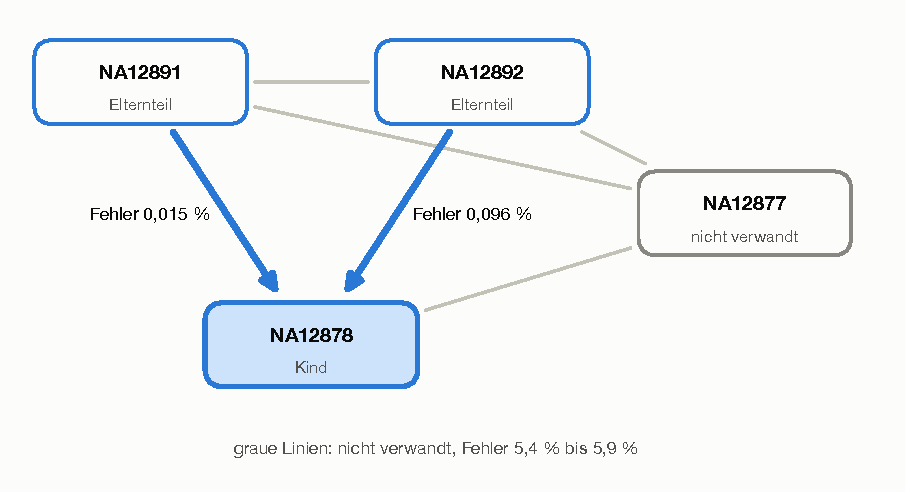
\includegraphics[width=\columnwidth]{abb1_verwandtschaftsnetz.pdf}
\caption{Abgeleitete Verwandtschaft. Die Pfeile gehen von den Eltern zum Kind, die Zahlen sind die Mendel-Fehlerraten.}
\label{fig:netz}
\end{figure}

\begin{figure}[t]
\centering
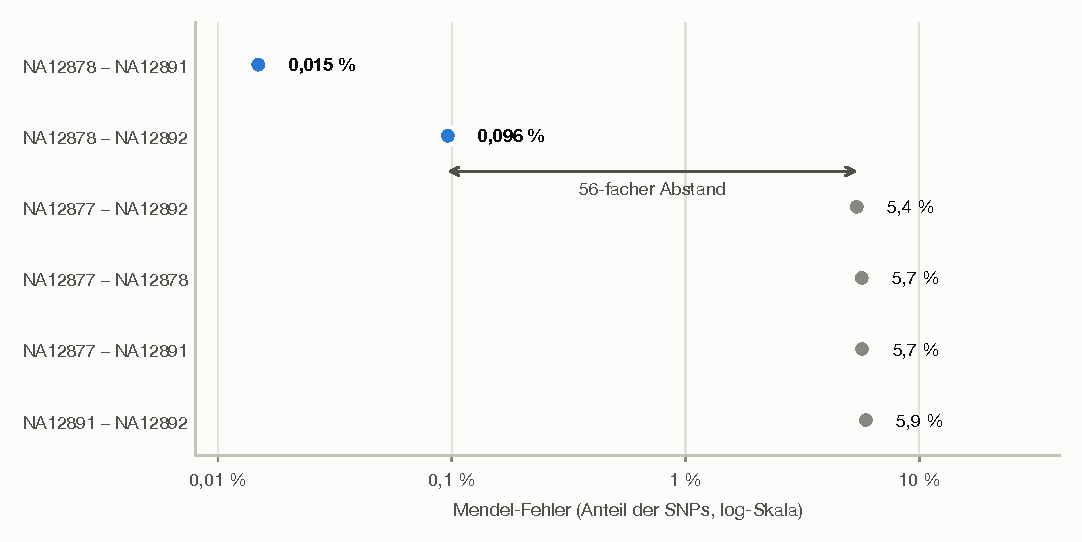
\includegraphics[width=\columnwidth]{abb2_mendel_paare.pdf}
\caption{Mendel-Fehlerrate pro Paar (logarithmische Skala).}
\label{fig:paare}
\end{figure}

\begin{figure}[t]
\centering
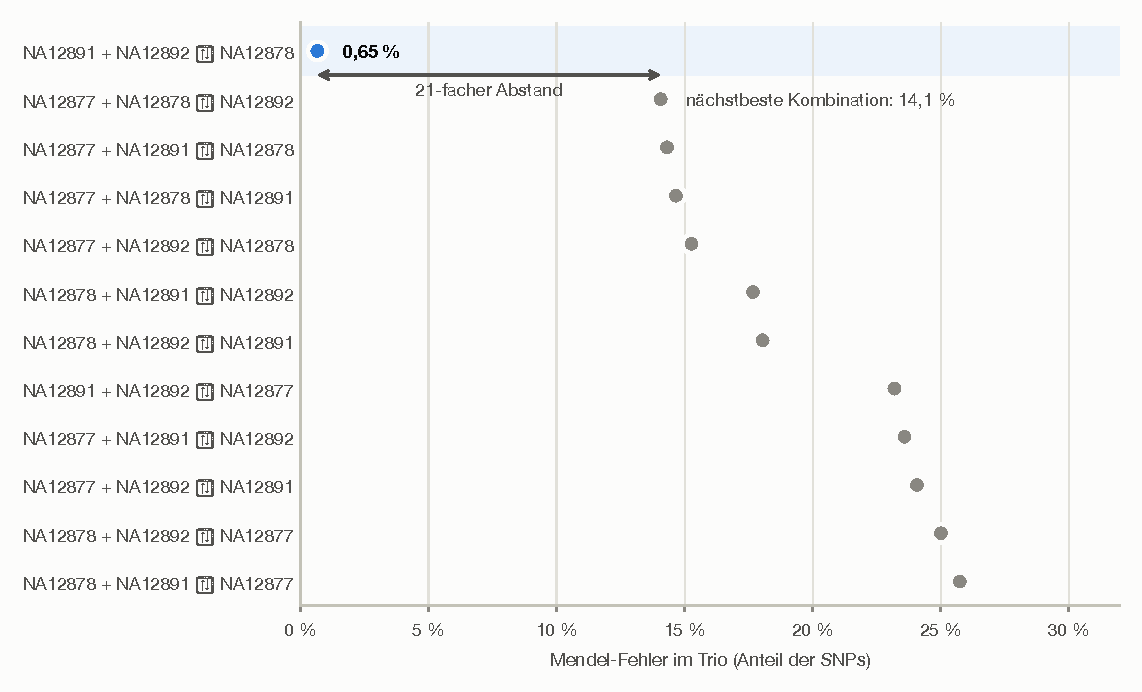
\includegraphics[width=\columnwidth]{abb3_mendel_trios.pdf}
\caption{Mendel-Fehlerrate aller zwölf Trio-Kombinationen. Das beste Trio ist blau hervorgehoben.}
\label{fig:trios}
\end{figure}

\begin{figure}[t]
\centering
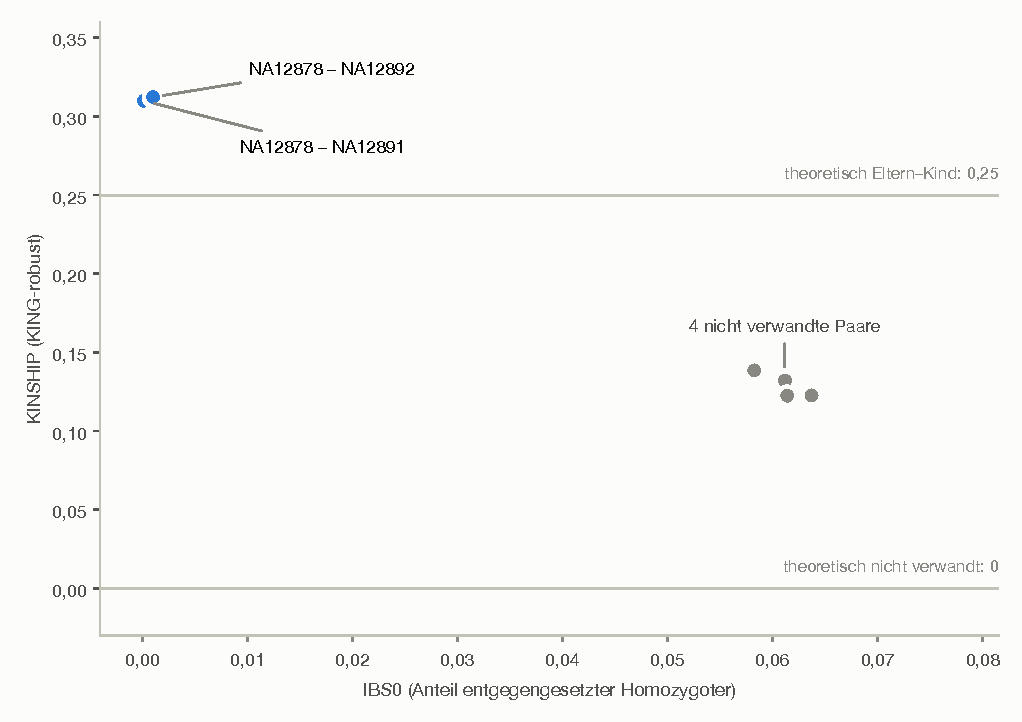
\includegraphics[width=\columnwidth]{abb4_king.pdf}
\caption{KING: IBS0 gegen KINSHIP. Die waagerechten Linien zeigen die theoretischen Erwartungswerte (0,25 und 0).}
\label{fig:king}
\end{figure}

% ---------------------------------------------------------------------------
\section{Ausführung und Reproduktion}
Alle Befehle laufen im Projektordner mit aktivierter Umgebung.
\begin{lstlisting}
mkdir -p data work
snakemake -n
caffeinate -i snakemake -j 8 \
  --resources mem_gb=16 \
  --rerun-triggers mtime
python scripts/plot_results.py
\end{lstlisting}
\texttt{snakemake -n} ist ein Trockenlauf und zeigt, was laufen würde. \texttt{-j 8} erlaubt 8 gleichzeitige Kerne, \texttt{--resources mem\_gb=16} begrenzt den verplanten Speicher (die Regeln melden je 8~GB an), und \texttt{--rerun-triggers mtime} startet nur Regeln neu, deren Eingabe neuer ist als die Ausgabe. \texttt{caffeinate -i} hält den Mac wach. Ein einzelnes Ziel wird mit dem Dateinamen vor den Optionen gestartet, zum Beispiel \texttt{snakemake results/snps.vcf.gz --rerun-triggers mtime}.

Der Bericht und diese Dokumentation werden mit LaTeX übersetzt (die Dokumentation braucht BibTeX für die Literatur):
\begin{lstlisting}
pdflatex dokumentation.tex
bibtex dokumentation
pdflatex dokumentation.tex
pdflatex dokumentation.tex
\end{lstlisting}

% ---------------------------------------------------------------------------
\section{Fehlersuche}
\paragraph{\texttt{Failed to open work/cohort.log}.} Die Regel \texttt{king} schreibt nach \pf{work/}, aber Snakemake entfernt den Ordner, wenn nach dem Löschen der temporären BAM-Dateien nichts mehr darin liegt. Abhilfe: \texttt{mkdir -p work} und den Lauf wiederholen. Dauerhaft hilft ein \texttt{mkdir -p work} in der Regel \texttt{king} vor dem ersten \texttt{plink2}-Aufruf.

\paragraph{Snakemake will alles neu rechnen.} Nach Änderungen am \texttt{Snakefile} erkennt Snakemake die Regeln als geändert. Mit \texttt{--rerun-triggers mtime} werden nur Regeln wiederholt, deren Eingabe neuer ist als die Ausgabe. Vorher mit \texttt{snakemake -n} prüfen.

\paragraph{Das Ziel wird als Ressource gelesen.} \texttt{--resources} nimmt mehrere Werte entgegen. Ein Ziel nach dieser Option wird deshalb falsch gelesen. Das Ziel gehört vor die Optionen.

\paragraph{Download bricht ab.} Kurze Verbindungs- und DNS-Ausfälle (curl-Fehler 18 und 6) fängt die Regel \texttt{download\_fastq} selbst ab. Sie setzt fort und gibt nach 50 Versuchen auf. Bleibt der Fehler, später erneut starten.

\paragraph{Der Mac geht in den Ruhezustand.} Den Lauf mit \texttt{caffeinate -i} starten.

\paragraph{Im PDF erscheinen \texttt{(?)} statt Literatur.} Der BibTeX-Schritt ist nicht gelaufen. Die Kette \texttt{pdflatex}, \texttt{bibtex}, zweimal \texttt{pdflatex} ausführen und prüfen, dass \pf{literatur.bib} im selben Ordner liegt.

% ---------------------------------------------------------------------------
\section{Grenzen}
\begin{itemize}
  \item Es wurden nur drei Chromosomen und vier Personen untersucht. Die Aussage gilt für diese Daten.
  \item Vater und Mutter lassen sich mit autosomalen Daten nicht unterscheiden. Dafür wäre Chromosom~X nötig. Das Mendel-Skript überspringt haploide Aufrufe und müsste dafür angepasst werden.
  \item Die Genotypfilter (\texttt{min\_dp}, \texttt{min\_gq}) sind nicht kalibriert, und eine Rekalibrierung der Basenqualitäten (BQSR) ist nicht Teil der Pipeline.
  \item Die Ursache der verschobenen KINSHIP-Werte ist nicht geklärt.
  \item Die Abbildungsskripte sind nicht in Snakemake eingebunden und laufen von Hand.
\end{itemize}

\bibliographystyle{plainnat}
\bibliography{literatur}

\appendix
\section{Skripte}
\subsection*{Snakefile}\label{app:snake}
\lstinputlisting[language=Python]{Snakefile}
\subsection*{mendel\_check.py}
\lstinputlisting[language=Python]{scripts/mendel_check.py}
\subsection*{plot\_results.py}
\lstinputlisting[language=Python]{scripts/plot_results.py}

\end{document}
